\documentclass{article}

\usepackage{arxiv}

\usepackage[utf8]{inputenc} % allow utf-8 input
\usepackage[T1]{fontenc}    % use 8-bit T1 fonts
\usepackage{lmodern}        % https://github.com/rstudio/rticles/issues/343
\usepackage{hyperref}       % hyperlinks
\usepackage{url}            % simple URL typesetting
\usepackage{booktabs}       % professional-quality tables
\usepackage{amsfonts}       % blackboard math symbols
\usepackage{nicefrac}       % compact symbols for 1/2, etc.
\usepackage{microtype}      % microtypography
\usepackage{lipsum}
\usepackage{graphicx}

\title{Spatial Scales of Local Adaptation and Host-Parasite Coevolution}

\author{
    Bob Week
   \\
    Integrative Biology \\
    Michigan State University \\
  East Lansing, MI 48824 \\
  \texttt{\href{mailto:bobweek@gmail.com}{\nolinkurl{bobweek@gmail.com}}} \\
   \And
    Gideon Bradburd
   \\
    Integrative Biology \\
    Michigan State University \\
  East Lansing, MI 48824 \\
  \texttt{\href{mailto:bradburd@msu.edu}{\nolinkurl{bradburd@msu.edu}}} \\
  }


% Pandoc citation processing
\newlength{\csllabelwidth}
\setlength{\csllabelwidth}{3em}
\newlength{\cslhangindent}
\setlength{\cslhangindent}{1.5em}
% for Pandoc 2.8 to 2.10.1
\newenvironment{cslreferences}%
  {}%
  {\par}
% For Pandoc 2.11+
\newenvironment{CSLReferences}[3] % #1 hanging-ident, #2 entry spacing
 {% don't indent paragraphs
  \setlength{\parindent}{0pt}
  % turn on hanging indent if param 1 is 1
  \ifodd #1 \everypar{\setlength{\hangindent}{\cslhangindent}}\ignorespaces\fi
  % set entry spacing
  \ifnum #2 > 0
  \setlength{\parskip}{#2\baselineskip}
  \fi
 }%
 {}
\usepackage{calc} % for calculating minipage widths
\newcommand{\CSLBlock}[1]{#1\hfill\break}
\newcommand{\CSLLeftMargin}[1]{\parbox[t]{\csllabelwidth}{#1}}
\newcommand{\CSLRightInline}[1]{\parbox[t]{\linewidth - \csllabelwidth}{#1}}
\newcommand{\CSLIndent}[1]{\hspace{\cslhangindent}#1}

\usepackage{amsmath}
\usepackage{dutchcal}
\usepackage{mathrsfs}
\usepackage{csquotes}
\usepackage{textcomp}
\usepackage[T3,T1]{fontenc}
\DeclareSymbolFont{tipa}{T3}{cmr}{m}{n}
\DeclareMathAccent{\invbreve}{\mathalpha}{tipa}{16}


\begin{document}
\maketitle

\def\tightlist{}


\begin{abstract}
Studies of local adaptation between coevolving hosts and parasites have
profited from theory that assumes a discrete set of populations.
However, when dispersal is limited continuous patterns of phenotypic
variation may emerge. Thus, patterns of local adaptation may occur on
characteristic spatial scales determined by relative dispersal distances
and strengths of selection. Furthermore, neutral patterns of spatial
correlation between traits may occur when they are spatially
autocorrelated. Hence, theory is needed to understand spatial scales of
local adaptation and coevolution and to disentangle the causes of
patterns of trait correlations across space. To fill this gap we study a
two-dimensional continuous space model of host-parasite coevolution. Our
results synthesize theory of host-parasite coevolution, local adaptation
and evolution in continuous space by \ldots{} We find that the species
with more limited dispersal tend to be locally adapted, but XYZ about it
being ahead in the coevolutionary race. To verify our results when model
assumptions are broken, we use individual based simulations. We find XYZ
about our results when coevolution is strong and XYZ when population
densities significantly vary across space.
\end{abstract}

\keywords{
    host-parasite coevolution
   \and
    local adaptation
   \and
    continuous space
   \and
    characteristic scales
   \and
    spde
  }

\hypertarget{introduction}{%
\section{Introduction}\label{introduction}}

Local adaptation occurs when individuals reared in the same geographic
location as their ancestors exhibit higher fitness than when reared
elsewhere. This phenomenon is thought to occur (or has been show to
occur) when selection is spatially heterogeneous and strong relative to
dispersal (refs).

\begin{itemize}
\item
  It seems an old motivation for studying local adaptation in
  host-parasite coevolution comes from trying to make sense of the GMTC.
  So I think it would be good to include this.
\item
  Need to do lit review of local adaptation in coevolving host-parasite
  systems.
\item
  We should also tie in previous work on understand spatial scales of
  phenotypic variation (ie, Slatkin's 1978 ppr). Need to do lit review
  in this area too.
\end{itemize}

\hypertarget{methods}{%
\section{Methods}\label{methods}}

To understand patterns of phenotypic variation and local adaptation in
continuous space, we introduce and analyze a pair of stochastic partial
partial differential equations (SPDE) that account for coevolution
between host and parasite, abiotic stabilizing selection and random
genetic drift. In particular, SPDE are stochastic generalizations of
deterministic PDE which in turn have been widely employed in theoretical
evolutionary ecology to study continuous space population dynamics
(refs), the evolution of continuous trait distributions (refs) and
feedbacks between the two (refs). Here we employ the SPDE framework to
model the evolution of mean traits in coevolving hosts and parasites. By
assuming additive genetic variances and population sizes are spatially
and temporally homogeneous, we arrive at a pair of linear SPDE driven by
space-time white noise processes. Linearity of the model allows us to
employ spectral methods to approximate spatial auto-covariance functions
of mean traits for each species along with a spatial cross-covariance
function between the mean traits of the two species. Using the spatial
auto-covariance functions, we then identify spatial scales of phenotypic
turnover.

In section \ref{spde} we introduce our model and briefly outline our
approach using spectral methods. More information on this approach is
provided in Appendix \ref{spde-app}. We then adapt a classical measure
of local adaptation in terms of population growth rates instead of
fitness measured as lifetime reproductive output. Using these adapted
measures, we apply our model results to illustrate the spatial scales of
local adaptation and to determine which species has a coevolutionary
advantage. These definitions are provided in section \ref{la} and
further details are located in Appendix \ref{la-app}. To test our
analytical results, we employ individual-based simulations conducted in
the language Julia (ref). In section \ref{ibs}, we provide a brief
overview of our simulation model. Further details on the
individual-based model can be found in Appendix \ref{ibs-app}

\hypertarget{spde-model}{%
\subsection{\texorpdfstring{SPDE model
\label{spde}}{SPDE model }}\label{spde-model}}

We employ a pair of stochastic partial differential equations to track
the evolution of mean traits in the host, \(\bar z_H(\pmb x)\), and the
parasite, \(\bar z_P(\pmb x)\), as functions of the two-dimensional
spatial coordinates \(\pmb x=(x_1,x_2)^\top\). We assume geographical
space is unbounded so that \(\pmb x\) spans the entire plane
\(\mathbb R^2\). We account for the effects of host-parasite coevolution
using a trait-matching model (ref other pprs using this model). Under
this model, fitness of the host is minimized and fitness of the parasite
is maximized when traits are matching. This induces a local
coevolutionary chase, where the parasite evolves to match the host, but
the host evolves to escape the parasite (this should be stated in the
introduction somewhere). The strength of biotic selection (i.e.,
selection that is induced by the interaction between hosts and
parasites) is denoted by \(B_H>0\) for the host and \(B_P>0\) for the
parasite. We assume these strengths of selection are temporally and
spatially homogeneous. To obtain an equilibrium solution to our model,
we also account for the effects of abiotic stabilizing selection. Here,
we assume abiotic optimal traits and strengths of abiotic selection for
both species are temporally and spatially homogeneous. We denote by
\(\theta_H,\theta_P\) the abiotic optimal traits and by \(A_H,A_P>0\)
the strengths of abiotic stabilizing selection in the host and parasite
respectively. Finally, our model also accounts for the effects of
limited dispersal by assuming individuals disperse following a bivariate
Gaussian distribution with mean zero and equal standard deviations in
both directions. We denote by \(\sigma_H,\sigma_P>0\) the standard
deviations of individual movement in the host and parasite respectively.
In our SPDE model, this translates to diffusion with coefficients
\(\sigma_H/2\) and \(\sigma_P/2\) (refs). For the sake of mathematical
tractability, we also assume the additive genetic variances
\(G_H,G_P>0\) and population densities \(\rho_H,\rho_P>0\) are
temporally and spatially homogeneous for the host and parasite
respectively. In Table X we provide a summary of model parameters. With
this notation, our model can be written as

\begin{subequations}\label{spde-model}
  \begin{equation}
    \frac{\partial\bar z_H}{\partial t}=G_HB_H(\bar z_H-\bar z_P)+G_HA_H(\theta_H-\bar z_H)+\frac{\sigma_H}{2}\left(\frac{\partial^2\bar z_H}{\partial x_1^2}+\frac{\partial^2\bar z_H}{\partial x_2^2}\right)+\sqrt\frac{G_H}{\rho_H}\dot W_H,
  \end{equation}
  \begin{equation}
    \frac{\partial\bar z_P}{\partial t}=G_PB_P(\bar z_H-\bar z_P)+G_PA_P(\theta_P-\bar z_P)+\frac{\sigma_H}{2}\left(\frac{\partial^2\bar z_P}{\partial x_1^2}+\frac{\partial^2\bar z_P}{\partial x_2^2}\right)+\sqrt\frac{G_P}{\rho_P}\dot W_P.
  \end{equation}
\end{subequations}

Here \(\dot W_H,\dot W_P\) denote two independent space-time white noise
processes, which are Gaussian processes with values that are independent
in both space and time. In particular, integrating \(\dot W_S\), (for
either \(S=H\) or \(S=P\)), over an interval of time \([t_1,t_2]\) and a
geographic region \(U\) returns a normally distributed random variable
with mean zero and variance equal to \((t_2-t_1)|U|\), where \(|U|\)
denotes the area of \(U\) (refs). Hence, over an interval of unit length
and region of unit area, the integral of \(\sqrt{G_S/\rho_S}\dot W_S\)
is normal with mean zero and variance \(G_S/\rho_S\) in analogy with
classical models of random genetic drift used in quantitative genetic
theory (refs). Since every parameter of the model is assumed to be
spatially and temporally homogeneous, spatial variation under this model
is ultimately caused by random genetic drift.

The assumption of constant effective population size across time and
space can be thought of as an extreme form of population regulation.
However, the model is agnostic to whether population regulation is
caused by top-down forces such as predation, bottom-up forces such as
resource competition or some combination thereof. Similarly, the
assumption of constant additive genetic variances can be justified
theoretically via mutation-selection balance (refs).

We analyze model (\ref{spde-model}) at its statistical equilibrium,
which exists and is unique when \(A_H>B_H\) (see Appendix
\ref{spde-app}). Following well established results of spatial
statistics (refs), we know the equilibrium solution of model
(\ref{spde-model}) is a bivariate Gaussian random field (refs for GRFs).
An example of an equilibrium solution to model (\ref{spde-model}) is
illustrated in Figure X. A multivariate Gaussian random field of \(p\)
variables has the convenient property of being characterized by its
\(p\)-dimensional mean vector \(\pmb \mu(x_1,x_2)\) and \(p\times p\)
spatial auto/cross-covariance matrix \(\pmb C(\pmb x,\pmb y)\) (refs).
While the (intraspecific) auto-covariance functions for each of the
\(p\) variables occur along the diagonal of \(\pmb C(\pmb x,\pmb y)\),
the (interspecific) cross-covariance functions occur on the off-diagonal
entries representing covariance between different variables at
potentially different locations. In particular, the \((i,j)\)th entry of
\(\pmb C(\pmb x,\pmb y)\) measures the covariance between the \(i\)th
and \(j\)th variables sampled at locations \(\pmb x=(x_1,x_2)\) and
\(\pmb y=(y_1,y_2)\) respectively. Taking expectation of our model at
equilibrium, we find \(\pmb\mu(x_1,x_2)=(\tilde z_H,\tilde z_P)^\top\)
is the vector of expected equilibrium trait values, which are spatially
homogeneous and are determined by a balance between biotic and abiotic
selection (expressions and derivation are provided in Appendix
\ref{spde-app}).

Obtaining the spatial auto/cross-covariance matrix
\(\pmb C(\pmb x,\pmb y)\) is more challenging. However, since we assume
all model parameters are spatio-temporally homogeneous, we can use known
results on linear SPDE to conclude that \(\pmb C(\pmb x,\pmb y)\) is
stationary which implies that it only depends on the distance between
\(\pmb x\) and \(\pmb y\) (refs). Hence, from hereon we write
\(\pmb C(d)\) for some distance \(d\geq0\) between sampled locations.
Linearity of the SPDE model (\ref{spde-model}) and stationarity of the
auto/cross-covariance matrix allow us to employ spectral methods and
capitalize on the relationship between spatial auto-covariance functions
and power spectra of stationary Gaussian random fields. In particular,
the power spectrum of a stationary Gaussian random field (where
stationarity here implies spatial homogeneity of mean vector and
stationarity of auto-covariance function) is the Fourier transform of
the spatial auto-covariance function. Denote by
\((\hat z_H(\pmb k),\hat z_P(\pmb k))^\top=\mathcal F\big[(\tilde z_H(\pmb x),\tilde z_P(\pmb x))^\top\big]\)
the Fourier transformed equilibrium solution to model
(\ref{spde-model}), where \(\pmb k=(k_1,k_2)\) correspond to spatial
frequencies in each direction. The power spectra of the stationary
solution to our model can then be computed as
\(S_H(\pmb k)=\mathbb E(\hat z_H^2(\pmb k))\),
\(S_P(\pmb k)=\mathbb E(\hat z_P^2(\pmb k))\) and
\(S_{HP}(k)=\mathbb E(\hat z_H(\pmb k)\hat z_P(\pmb k))\), where
\(\mathbb E\) denotes expectation across all possible outcomes. Then, by
setting \(C_H(d), C_P(d)\) equal to the respective spatial
auto-covariance functions of the host and parasite mean traits and
\(C_{HP}(d)\) equal to the spatial cross-covariance function between
host and parasite mean traits, we have

\begin{equation}
  C_H(d) = \mathcal F^{-1}\big[S_H(\pmb k)\big], \ C_P(d) = \mathcal F^{-1}\big[S_P(\pmb k)\big], \ C_{HP}(d)=\mathcal F^{-1}\big[S_{HP}(\pmb k)],
\end{equation}

where \(\mathcal F^{-1}\) denotes inverse Fourier transformation. Hence,
although directly calculating the matrix of spatial covariance functions
\(\pmb C(d)\) from model (\ref{spde-model}) is challenging, computing
the power spectra and taking their inverse Fourier transforms is
straightforward when the power spectra take simple forms. In Appendix
\ref{spde-app} we use a weak coevolution approximation to simplify
expressions of power spectra and calculate analytical expressions for
the spatial (intraspecific) auto-covariance and (interspecific)
cross-covariance functions of host and parasite mean traits. In the next
section, we make use of the spatial cross-covariance function
\(C_{HP}(d)\) to define a measure of local adaptation for species
distributed continuously in space.

\hypertarget{local-adaptation-in-continuous-space}{%
\subsection{\texorpdfstring{Local adaptation in continuous space
\label{la}}{Local adaptation in continuous space }}\label{local-adaptation-in-continuous-space}}

Measures of local adaptation quantify the difference in average fitness
of individuals reared in local environmental conditions versus average
fitness of individuals reared in foreign environmental conditions
(refs). When individual fitness tends to be greater in local conditions
in comparison to foreign conditions, the species is considered to be
locally adapted. In this section we introduce a definition of local
adaptation for species distributed continuously in space. However,
before doing so, we briefly review a classical measure of local
adaptation for species distributed in a finite number of discrete
locations to motivate our continuous space analog.

Classically, measures of local adaptation are defined for finite,
spatially discrete habitats in terms of expected lifetime reproductive
output for an average individual transplanted from some locality \(i\)
to some other locality \(j\), denoted here by \(\bar w_S(i,j)\) for
species \(S=H,P\). The bar above \(w_S\) signifies that we are averaging
across trait values of individuals in species \(S\) found at location
\(i\). Then, assuming a finite number \(K\) of discrete habitats,
average fitness of individuals reared in their local environmental
conditions can be captured by \(\bar{\bar w}_S=\sum_i\bar w_S(i,i)/K\)
and average fitness of individuals transplanted to a randomly selected
location can be captured by
\(\hat{\bar w}_S=\sum_{i,j }\bar w_S(i,j)/K^2\), where the sums are
taken over \(i=1,\dots,K\) and \(i,j=1,\dots,K\) respectively. Then, a
commonly used definition of local adaptation is given by
\(\mathcal L_S=\bar{\bar w}_S-\hat{\bar w}_S\) (refs). In turn,
\(\mathcal L_S\) can be written in terms of the spatial covariance of
host and parasite genotype frequencies (refs) or of host and parasite
phenotypic distributions (see Appendix \ref{}). In particular, this
definition implies the parasite species is locally adapted when genotype
or phenotype frequencies between host and parasite positively covary
across locations. Conversely, the host is locally adapted when this
covariance is negative.

To obtain an analogous measure of local adaptation to \(\mathcal L_S\)
for species distributed continuously in space, we consider the
difference in Malthusian growth rates for individuals reared in local
conditions versus those reared in randomly drawn locations. In
particular, we denote by \(m_H(z_H,z_P)\) the Malthusian growth rate of
host individuals having trait \(z_H\) encountering parasite individuals
with trait \(z_P\). Similarly, \(m_P(z_P,z_H)\) is the growth rate of
parasite individuals with trait \(z_P\) encountering host individuals
with trait \(z_H\). Setting \(\varphi_S(z_S,\pmb x)\) the frequency of
trait value \(z_S\) in species \(S\) at location \(\pmb x\), the
Malthusian growth rate of hosts transplanted from location \(\pmb x\) to
location \(\pmb y\) is given by

\begin{equation}
  \bar m_H(\pmb x,\pmb y)=\int_{-\infty}^{+\infty}\int_{-\infty}^{+\infty}m_H(z_H,z_P)\varphi_H(z_H,\pmb x)\varphi_P(z_P,\pmb y)dz_Hdz_P.
\end{equation}

The analogous quantity for the parasite species,
\(\bar m_P(\pmb x,\pmb y)\), can be defined in a similar fashion. Since,
under our model (\ref{spde-model}), mean traits are random variables,
the Malthusian growth rates
\(\bar m_H(\pmb x,\pmb y),\bar m_P(\pmb x,\pmb y)\) are also random
variables. We therefore define local adaptation in terms of expectations
of these growth rates. In particular, we define a geographically
specific measure of local adaptation for individuals of species \(S\)
drawn from location \(\pmb x\) and transplanted to location \(\pmb y\)
as

\begin{equation}
  \Delta_S(\pmb x,\pmb y)=\mathbb E\big[\bar m_S(\pmb x,\pmb x)-\bar m_S(\pmb x,\pmb y)\big].
\end{equation}

Since our model of mean trait evolution described in section \ref{spde}
implies \((\bar z_H(\pmb x),\bar z_P(\pmb x))^\top\) is a stationary,
isotropic Gaussian random field, \(\bar m_S(\pmb x,\pmb y)\) and
\(\Delta_S(\pmb x,\pmb y)\) depend only on the distance \(d\geq0\)
between locations \(\pmb x\) and \(\pmb y\) for both host and parasite.
We therefore write \(\bar m_S(d)=\bar m_S(\pmb x,\pmb y)\) and
\(\Delta_S(d)=\Delta_S(\pmb x,\pmb y)\) when the distance between
\(\pmb x\) and \(\pmb y\) is \(d\). Furthermore, since we model host and
parasite species as being distributed continuously across the entire
plane \(\mathbb R^2\), the assumption that the location transplanted to
is drawn uniformly at random (consistent with the classical measure
\(\mathcal L_S\)) implies the distance transplanted will almost surely
be infinite. We therefore define our continuous space analog of local
adaptation for species \(S\) as

\begin{equation}\label{la-cont-sp}
  \ell_S=\lim_{d\to\infty}\Delta_S(d).
\end{equation}

In section \ref{} we present results found by combining our definition
of local adaptation in continuous space with our model of host-parasite
coevolution. Although this definition and analytical results presented
below have relatively simple expressions, they come at the cost of
several important model assumptions. We therefore developed
individual-based simulations to relax these key assumptions. In the
following section, we describe the structure of our individual-based
simulations and approach taken to analyze simulated output for
comparison with results found using the SPDE model (\ref{spde-model}).

\hypertarget{relaxing-model-assumptions}{%
\subsection{\texorpdfstring{Relaxing model assumptions
\label{ibs}}{Relaxing model assumptions }}\label{relaxing-model-assumptions}}

To understand the robustness of our results, we developed
individual-based simulations that relax key model assumptions. In
particular, we investigated the consequences of relaxing the assumptions
of weak coevolution and unbounded habitat along with spatio-temporally
homogeneous population densities, additive genetic variances and abiotic
optimal trait values. In this section we begin by describing the
structure of our individual-based models, our approach taken to
implement or relax key assumptions and methods used to assess the
robustness of our analytical results.

\hypertarget{individual-based-simulations}{%
\subsubsection{Individual-based
simulations}\label{individual-based-simulations}}

In each of our individual-based simulations, we track the dynamics of
host and parasite species consisting of a finite number of individuals
distributed on the unit square. We assume discrete, non-overlapping
generations so that time can be measured in integral steps. At the
beginning of each generation, we accumulate consequences of intra and
interspecific interactions on the fitness of individuals. In particular,
we assume a spatial competition model where individual fitness is
reduced multiplicatively by an amount \(0<\kappa_S<1\) for each
conspecific within a radius \(R_S>0\), where both of these parameters
depend on the species \(S\). For example, if the base fitness of a host
individual located at \(\pmb x\) is \(w\) and there are \(n\) other
hosts within \(R_H\) of \(\pmb x\), the resulting fitness of this host
individual after spatial competition is \(w'=w\times(\kappa_H)^n\).
Interspecific interactions between host and parasite individuals are
modeled in a similar fashion. We assume parasites choose a single host
at random from within a radius \(R_\iota>0\) of the focal parasite
location. The probability of infection \(\pi(z_H,z_P)\) is determined by
the degree to which host and parasite traits match, with a maximum
probability of infection \(\pi_{\max}>0\) occurring when \(z_H=z_P\).
The rate at which the probability of infection decays with \(|z_H-z_P|\)
is mediated by \(\gamma>0\). When infection fails, we assume no
consequences for the fitnesses of individuals involved. In the case of
successful infection, we assume the host incurs a fitness cost of
\(0<\iota_H<1\) and the parasite receives a fitness benefit of
\(\iota_P>1\). To decouple the effects of spatial competition from
coevolution, we allow multiple parasites to infect the same host. Then,
given a base fitness of \(w\) for a host individual being infected by
\(n\) parasites, the updated host fitness becomes
\(w'=w\times(\iota_H)^n\). Finally, we incorporate abiotic stabilizing
selection on each species. In particular, individuals accumulate
multiplicative fitness effect \(\mathcal A_S(z_S,\theta_S)\) that
depends on the difference \(|z_S-\theta_S|\) where \(\theta_S\) is the
abiotic optimal trait for species \(S\) and may depend on geographical
location. The maximum fitness effect due to the abiotic environment is
\(\alpha_S>0\) and occurs when \(z_S=\theta_S\). The rate at which
\(\mathcal A_S(z_S,\theta_S)\) decays with \(|z_S-\theta_S|\) is
mediated by \(a_S>0\). Before fitness effects are accumulated, we assume
all host and parasite individuals begin with a base fitness of one.
Population densities can be controlled by tuning the fitness effects of
spatial competition \(\kappa_H,\kappa_P\), interspecific interactions
\(\iota_H,\iota_P\), the maximum fitness effects of abiotic selection
\(\alpha_H,\alpha_P\) and the interaction radii \(R_H,R_P,R_\iota\).

At the end of each generation each individual is replaced by a random
number of offspring. In particular, for an individual that has
accumulated a fitness of \(w\), the number of offspring is drawn from a
Poisson distribution with mean \(w\). Trait values of offspring are
normally distributed around parental values with variance \(\mu_S\) for
species \(S\). For simplicity, we assume traits are perfectly heritable.
Geographical locations of individuals are also normally distributed
(bivariate normal in particular) around parental locations with standard
deviation in each direction \(\sigma_S\) for species \(S\). If an
offspring location falls outside the unit square, one of three
possibilities occur depending on the boundary conditions chosen. For
absorbing boundary conditions, the offspring is removed from the
population. For reflecting boundary conditions, the offspring bounces
off the habitat boundary with symmetric angles of incidence and
reflection. Multiple bounces are possible until the offspring travels
the same distance as it would in the absence of boundaries. In the case
of periodic boundaries, an offspring that falls off the edge of the
habitat appears on the opposite side as if the habitat boundaries were
connected to form a torus. Note that spatial competition prevents the
famed \emph{pain in the torus} problem (refs). The boundary conditions
chosen (e.g., absorbing, reflecting or periodic) for a given simulation
depended on whether or not that simulation was developed for
investigating the effects of geographically bounded habitats.

This concludes the general description of our simulation model. Further
details can be found in Appendix \ref{} (including details on spatially
heterogeneous abiotic optima). Simulation model parameters are
summarized in Table Y. Code for simulations were written in the language
\emph{Julia} (Bezanson et al. 2017) and can be found in the github
repository
\url{https://github.com/bobweek/continuous-space-coevolution}. In the
next subsection, we describe our use of this simulation model to check
the robustness of our analytical results.

\hypertarget{assessing-robustness-of-analytical-results}{%
\subsubsection{Assessing robustness of analytical
results}\label{assessing-robustness-of-analytical-results}}

To assess the robustness of our analytical results in face of broken
assumptions, we quantified spatial scales of phenotypic turnover and
local adaptation for simulated populations. We then compared the
simulated results to analytical results. In particular, to simplify
comparison with analytical results, we fitted Matérn spatial correlation
functions to simulated trait data separately for each species. To do
this, we first implemented a non-parametric estimator of the spatial
correlation function using the \emph{R} package \texttt{ncf} (Bjørnstad
and Bascompte 2001). We then used the \emph{R} function \texttt{optim}
to find a least squares approximation of the non-parametric estimator
across all parameter combinations of the Matérn correlation functions.
Matérn correlation functions are parameterized by a characteristic
length \(\xi\) and a roughness parameter \(\nu\). Hence, this approach
allowed us to estimate characteristic lengths of phenotypic turnover for
direct comparison with analytical results. However, before making such
comparisons we first assessed whether a Matérn correlation function
adequately describes the simulated data using a randomization test. In
the case that the simulated data significantly differed from a Matérn
correlation function, we concluded that our analytical result failed for
that region of model parameters and set of assumptions broken. In the
case that the simulated did not significantly differ from a Matérn
correlation function, we then used a randomization test to determine
whether or not the analytically predicted spatial scale of phenotypic
turnover is a good approximation of the simulated spatial scale of
phenotypic turnover. We did this for each species separately.

Next, we tested our results on local adaptation and coevolutionary
advantage.

\hypertarget{results}{%
\section{Results}\label{results}}

\hypertarget{spatial-covariances-and-characteristic-lengths-of-phenotypic-turnover}{%
\subsection{Spatial covariances and characteristic lengths of phenotypic
turnover}\label{spatial-covariances-and-characteristic-lengths-of-phenotypic-turnover}}

Using a weak coevolution approximation to simplify expressions for the
power spectra (see Appendix \ref{spde-app}), we were able to employ an
inverse Fourier transform to obtain analytic expressions for the
(intraspecific) spatial auto-covariance and (interspecific) spatial
cross-covariance functions of host and parasite mean trait values. In
particular, we find cross-covariance functions for the host and parasite
respectively taking the forms

\begin{subequations}
  \begin{equation}
    C_H(d)\approx\sqrt2V_H\frac{d}{\xi_H}K_1\left(\sqrt2\frac{d}{\xi_H}\right),
  \end{equation}
  \begin{equation}
    C_P(d)\approx\sqrt2V_P\frac{d}{\xi_P}K_1\left(\sqrt2\frac{d}{\xi_P}\right),
  \end{equation}
\end{subequations}

where \(V_H,V_P\) are the collocated variances (i.e., \(C_S(0)=V_S\) for
\(S=H,P\)), \(\xi_H,\xi_P\) are the characteristic lengths of phenotypic
turnover across geographic space in each species and \(K_\nu(d)\) is a
modified Bessel function of second order, degree \(\nu\) (ref
aboromitz). These spatial covariance functions belong to the class of
Matern covariance functions which have been widely employed in the
fields of spatial statistics (refs) and machine learning (refs).

The collocated variances \(V_H,V_P\) represent uncertainty in mean trait
value at any particular location as opposed to variance of trait values
among individuals at that location. Hence, mean traits of species \(S\)
(where \(S=H\) or \(S=P\)) at locations separated by distances much
greater than the characteristic length \(\xi_S\) returns essentially
independent and identically distributed random variables with variances
equal to the collocated variance \(V_S\). Thus, the collocated variances
also provide measures of global diversity of mean traits across space.
In terms of our model parameters, the collocated variances can be
expressed as

\begin{equation}
  V_H = \frac{1}{\rho_H\sigma_H^2(A_H-B_H)}, \ V_P = \frac{1}{\rho_P\sigma_P^2(A_P+B_P)}.
\end{equation}

From the expressions for \(V_H\) and \(V_P\) we see population density
\(\rho_S\), dispersal distance \(\sigma_S\) and strength of abiotic
stabilizing selection \(A_S\) all tend to decrease the overall diversity
of mean traits of species \(S\) across space. Since our model assumes
the ultimate source of spatial variation in mean traits is random
genetic drift, this explains why increased population density erodes
spatial diversity. Similarly, since we assume space extends across the
entire plane \(\mathbb R^2\), in the limit of infinite dispersal
distance we arrive at a panmictic population of infinite size,
explaining why increased \(\sigma_S\) decreases \(V_S\). These two
results mirror those found in studies of continuous space population
genetics using Wright's neighborhood size
\(\mathscr N_S=4\pi\rho_S\sigma_S\), which is a continuous space analog
of effective population size (refs). Since the abiotic optima
\(\theta_H,\theta_P\) are assumed to be spatially homogeneous, abiotic
stabilizing selection around these optima erodes spatial variation of
mean traits in both species. In contrast, biotic selection has opposing
effects on the degree of spatial variation in host and parasite mean
traits. In particular, while increased biotic selection erodes spatial
diversity of mean traits for the parasite species since it is
stabilizing under the trait-matching model, increased biotic selection
on the host promotes spatial variation because it is disruptive under
the trait-matching model. However, since we require abiotic stabilizing
selection on the host to outweigh biotic disruptive selection (i.e.,
\(A_H>B_H\)) for the existence of equilibrium solutions, selection will
be overall stabilizing for both species around augmented optima that
strike a balance between biotic and abiotic selection (see Appendix
\ref{spde-app}). In turn, since these augmented optima are spatially
homogeneous, the overall stabilizing effect of selection diminishes the
magnitude of spatial variation in mean traits for both species.

The characteristic lengths of phenotypic turnover across space in the
host and parasite can be expressed in terms of model parameters
respectively as

\begin{equation}\label{char-len}
  \xi_H = \frac{\sigma_H}{\sqrt{G_H(A_H-B_H)}}, \ \xi_P = \frac{\sigma_P}{\sqrt{G_P(A_P+B_P)}}.
\end{equation}

From these expressions, we see that characteristic spatial scales of
phenotypic variation are proportional to the standard deviations of
dispersal distances in the respective species. Hence, the further
individuals tend to move, the larger the spatial scales one must observe
to see significant phenotypic variation. We also see that increased
additive genetic variance and abiotic stabilizing selection tends to
decrease these spatial scales in each species. This reduction in spatial
scale by additive genetic variance can be explained by the fact that
additive genetic variation inflates the effects of random genetic drift,
here assumed to be the ultimate source of spatial variation. With
increased spatial variation, one can observe significant changes in mean
trait values over shorter spatial scales. However, since stabilizing
selection homogenizes mean trait values across space, it is less obvious
why increased strength of abiotic selection should decrease spatial
scales of phenotypic turnover.

In contrast to the relatively simple expressions for the intraspecific
auto-covariance functions, the expression for the interspecific
cross-covariance function is rather cumbersome. In particular,
\(C_{HP}(d)\) can be approximated as the difference of two convolutions
when coevolution is weak, the expression for which is provided in
Appendix \ref{spde-app}. However, our measure of local adaptation (eqn.
\ref{la-eq}) requires only the collocated covariance \(C_{HP}(0)\). We
can therefore sidestep calculating the cross-covariance \(C_{HP}(d)\)
for \(d>0\). The collocated covariance \(C_{HP}(0)\) can be obtained via
spectral methods and the calculations for which are provided in Appendix
\ref{spde-app}. In particular, we find

\begin{multline}\label{collocated}
  C_{HP}(0)\approx \frac{G_HG_P}{\sigma_H^2\sigma_P^2}\frac{\xi_H^2\xi_P^2}{(\xi_H^2-\xi_P^2)^2}\left[\frac{B_P}{\rho_H\sigma_H^2}\Big(\xi_H^4+\xi_H^2\xi_P^2(\ln\xi_P^2-\ln\xi_H^2-1)\Big)\right. \\
  \left.-\frac{B_H}{\rho_P\sigma_P^2}\Big(\xi_P^4+\xi_H^2\xi_P^2(\ln\xi_H^2-\ln\xi_P^2-1)\Big)\right].
\end{multline}

In analogy to how the collocated variances \(V_H,V_P\) provide global
measures of mean trait variation across space within each species, the
collocated covariance \(C_{HP}(0)\) provides a global measure of mean
trait co-variation across space between the two species. Expression
(\ref{collocated}) implies that, when hosts and parasites exhibit
approximately equal spatial scales of phenotypic turnover (i.e., when
\(\xi_H\approx\xi\) and \(\xi_P\approx\xi\) for some \(\xi>0\)), the
collocated covariance is approximately

\begin{equation}
  C_{HP}(0)\approx \frac{\xi^4}{2}G_HG_P\left(\frac{B_P}{\rho_H\sigma_H^4\sigma_P^2}-\frac{B_H}{\rho_P\sigma_H^2\sigma_P^4}\right).
\end{equation}

Hence, in this limiting case, we see that increased selection on the
parasite over the host tends to increase spatial covariance of host and
parasite mean traits. The same pattern holds true for population
densities \(\rho_H,\rho_P\) and for the dispersal distances when
\(\sigma_H,\sigma_P>1\). In the next section we capitalize on these
results to understand patterns of host and parasite local adaptation.

\hypertarget{local-adaptation}{%
\subsection{Local adaptation}\label{local-adaptation}}

In Appendix \ref{} we show that the trait-matching model of fitness used
to obtain the mean trait dynamics described by equation
(\ref{spde-model}) implies that \(\Delta_H(d)\) and \(\Delta_P(d)\) can
be simplified to

\begin{subequations}
  \begin{equation}
    \Delta_H(d)=B_H\big(C_{HP}(d)-C_{HP}(0)\big)
  \end{equation}
  \begin{equation}
    \Delta_P(d)=B_P\big(C_{HP}(0)-C_{HP}(d)\big).
  \end{equation}
\end{subequations}

Finally, since under our model of host-parasite coevolution the
cross-covariance function \(C_{HP}(d)\) decays to zero as
\(d\to\infty\), our measure of local adaptation for each species
simplifies to

\begin{subequations}\label{la-eq}
  \begin{equation}
    \ell_H = -B_HC_{HP}(0),
  \end{equation}
  \begin{equation}
    \ell_P = B_PC_{HP}(0).
  \end{equation}
\end{subequations}

From equations (\ref{la-eq}), we see that the host is locally adapted
(\(\ell_H>0\)) when host and parasite mean traits are negatively
correlated across sufficiently long distances (i.e., when
\(C_{HP}(0)<0\)) and that the parasite is locally adapted when mean
traits are positively correlated across sufficiently long distances,
where sufficiently long distances here correspond to distances at which
intraspecific spatial autocorrelations of mean trait values are
negligible. Hence, this definition is consistent with the classical
measure \(\mathcal L_S\) defined for species distributed across discrete
patches.

\hypertarget{discussion}{%
\section{Discussion}\label{discussion}}

In the absence of biotic selection, our expressions for the
characteristic lengths of phenotypic turnover across space (eqns.
\ref{char-len}) coincide with the characteristic length found by Slatkin
(1978) in his pioneering work on the evolution of quantitative traits in
continuous space. Notably, while Slatkin assumed one-dimensional space
and discrete time, we assume two-dimensional space and continuous time.
Furthermore, while Slatkin assumed spatial variation in mean traits were
the result of spatially varying abiotic stabilizing selection, we assume
the ultimate source of spatial variation is due to the effects of random
genetic drift. Whether or not this coincidence sheds light on some
universal property of phenotypic variation across space or is merely a
mathematical artifact due to the approximation schemes employed remains
unclear.

Limitations of our approach include the assumption of weakly coevolving
hosts and parasites, spatially homogeneous abiotic trait optima,
strengths of selection, additive genetic variances and abundance
densities. Furthermore, in order for our model to have equilibrium
solutions, we require abiotic selection to be greater than biotic
selection (i.e., \(A_H>B_H\)).

\hypertarget{conclusion}{%
\section{Conclusion}\label{conclusion}}

\newpage

\appendix

\begin{center}
\Large{Appendix}
\end{center}

\hypertarget{calculating-the-covariance-and-cross-covariance-functions}{%
\section{\texorpdfstring{Calculating the covariance and cross-covariance
functions
\label{spde-app}}{Calculating the covariance and cross-covariance functions }}\label{calculating-the-covariance-and-cross-covariance-functions}}

Assuming the system has reached a statistical equilibrium, we make use
of a Fourier transform convert the model from geographic coordinates to
frequency coordinates, where the Fourier transformed solution represents
the spatial harmonic content of the solution to the SPDE model. We then
use the Fourier transformed model to construct so-called power spectra
of the solution, which are exactly the Fourier transformed spatial
auto-covariance functions. We then use a weak coevolution approximation
to simplify the power spectra so they can be inverted, arriving at
analytical expressions for the spatial auto-covariance functions. In
turn, the functional form of the spatial auto-covariance functions
allows the identification of spatial scales of phenotypic turnover.

To compute formula for the spatial (intraspecific) covariance and
(interspecific) cross-covariance functions, we make use of the relation
between the covariance functions and power spectra of random fields. In
particular, the power spectrum of a multivariate stationary random field
\(\pmb F(\pmb x)\), \(\pmb x=(x_1,x_2)\) being spatial location, is
defined by
\(S_{\pmb F}(\pmb k)=\mathbb E\left(\hat{\pmb F}(\pmb k)\hat{\pmb F}(\pmb k)^H\right)\)
where \(\hat{\pmb F}(\pmb k)\) is the Fourier transform of \(\pmb F\),
the symbol \(^H\) denotes Hessian transpose and \(\pmb k=(k_1,k_2)\) are
the Fourier transformed coordinates which represent the frequencies of
fluctuations across the two spatial dimensions. Hence, \(\hat{\pmb F}\)
represents the harmonic content of the process \(\pmb F\). The spatial
covariance function \(C_{\pmb F}(\pmb x)\) is just the inverse Fourier
transform of the power spectrum \(S_{\pmb F}(\pmb k)\).

Working with the power spectrum has the advantage of converting
differential equations into algebraic equations, making for a more
analytically tractable approach. Furthermore, due to the Fourier
relationship between \(C_{\pmb F}(\pmb x)\) and \(S_{\pmb F}(\pmb k)\),
we have the convenient properties
\(\int_{\mathbb R^2}C_{\pmb F}(\pmb x)d\pmb x=S_{\pmb F}(\pmb 0)\) and
\(\int_{\mathbb R^2}S_{\pmb F}(\pmb x)d\pmb x=C_{\pmb F}(\pmb 0)\). Both
of these properties will aid in calculating results on host-parasite
local adaptation.

Using \(\pmb k=(k_1,k_2)\) to denote spatial frequency (the Fourier
equivalent to spatial location \(\pmb x=(x_1,x_2)\)) and
\(\hat{\pmb z}(\pmb k)=(\hat z_H(\pmb k),\hat z_P(\pmb k))^\top\) to
denote the Fourier transforms of the equilibrium solution
\(\bar{\pmb z}(\pmb x)=(\bar z_H(\pmb x),\bar z_P(\pmb x))^\top\), the
Fourier transform of our model at equilibrium is

\[0=G_HA_H(\theta_H-\hat z_H)-G_HB_H(\hat z_P-\hat z_H)-\frac{\sigma_H^2}{2}\|\pmb k\|^2\hat z_H+\sqrt\frac{G_H}{N_H}\widehat{\dot W}_H,\]

\[0=G_PA_P(\theta_P-\hat z_P)+G_PB_P(\hat z_H-\hat z_P)-\frac{\sigma_P^2}{2}\|\pmb k\|^2\hat z_P+\sqrt\frac{G_P}{N_P}\widehat{\dot W}_P,\]

where \(\|\pmb k\|^2=k_1^2+k_2^2\) and \(\widehat{\dot W}_S\) is a
heuristic representation for the Fourier transform of the spatial white
noise \(\dot W_S\) for species \(S=H,P\). Since the mean vector for
equilibrium solution of the SPDE model is spatially homogeneous, we set
\(\theta_H=\theta_P=0\) without loss of generality. This is equivalent
to centering the solution by working with \(\tilde z_H=\bar z_H-\mu_H\)
and \(\tilde z_P=\bar z_P-\mu_P\) instead of \(\bar z_H\) and
\(\bar z_P\). The Fourier transformed SPDE model can be rewritten in
matrix form as

\[\mathscr H\hat{\pmb z}=\widehat{\dot{\pmb W}}\]

where
\(\widehat{\dot{\pmb W}}=\tfrac{1}{2\pi}\left(-\sqrt{\tfrac{G_H}{N_H}}\hat{\dot W}_H, -\sqrt{\tfrac{G_P}{N_P}}\hat{\dot W}_P\right)^\top\)
and

\[\mathscr H=\frac{1}{2\pi}\left(\begin{matrix}-G_HA_H+G_HB_H+\frac{\sigma_H^2}{2}\|\pmb k\|^2 & -G_HB_H \\ G_PB_P & -G_PA_P-G_PB_P+\frac{\sigma_P^2}{2}\|\pmb k\|^2\end{matrix}\right).\]

Since no complex numbers appear in the above expressions, the power
spectrum of the random field \(\bar{\pmb z}\) simplifies to
\(S_{\bar{\pmb z}}=\mathbb E\left(\hat{\pmb z}\hat{\pmb z}^\top\right)\).
Rearranging the above matrix equation, we find

\[\hat{\pmb z}=\mathscr H^{-1}\widehat{\dot{\pmb W}},\]

\[\hat{\pmb z}^\top=\widehat{\dot{\pmb W}}^\top\left(\mathscr H^\top\right)^{-1}.\]

Hence, the power spectrum of \(\bar{\pmb z}\) is

\[S_{\bar{\pmb z}}=\mathscr H^{-1}S_{\dot{\pmb W}}\left(\mathscr H^\top\right)^{-1}\]

where

\[S_{\dot{\pmb W}}=\mathbb E\left(\widehat{\dot{\pmb W}}\widehat{\dot{\pmb W}}^\top\right)=\frac{1}{(2\pi)^2}\left(\begin{matrix}G_H/N_H & 0 \\ 0 & G_P/N_P \end{matrix}\right)\]

is the power spectrum of the spatial white noise
\(\dot{\pmb W}=\left(-\sqrt{\tfrac{G_H}{N_H}}{\dot W}_H, -\sqrt{\tfrac{G_P}{N_P}}{\dot W}_P\right)^\top\).
Denoting \(S_H,S_P\) and \(S_{HP}\) the components of
\(S_{\bar{\pmb z}}\) corresponding to the host power spectrum, parasite
power spectrum and host-parasite cross-power spectrum we find

\[S_H(\pmb k)=\frac{B_H^2G_H^2\frac{G_P}{N_P}+\frac{G_H}{N_H}\big[G_P(A_P+B_P)+\frac{1}{2}\sigma_P^2\|\pmb k\|^2\big]^2}{\big\{B_HB_PG_HG_P+[G_H(A_H-B_H)+\frac{1}{2}\sigma_H^2\|\pmb k\|^2][G_P(A_P+B_P)+\frac{1}{2}\sigma_P^2\|\pmb k\|^2]\big\}^2},\]

\[S_P(\pmb k)=\frac{B_P^2G_P^2\frac{G_H}{N_H}+\frac{G_P}{N_P}\big[G_H(A_H-B_H)+\frac{1}{2}\sigma_H^2\|\pmb k\|^2\big]^2}{\big\{B_HB_PG_HG_P+[G_H(A_H-B_H)+\frac{1}{2}\sigma_H^2\|\pmb k\|^2][G_P(A_P+B_P)+\frac{1}{2}\sigma_P^2\|\pmb k\|^2]\big\}^2},\]

\[S_{HP}(\pmb k)=\frac{B_PG_P\frac{G_H}{N_H}\big[G_P(A_P+B_P)+\frac{1}{2}\sigma_P^2\|\pmb k\|^2\big]-B_HG_H\frac{G_P}{N_P}\big[G_H(A_H-B_H)+\frac{1}{2}\sigma_H^2\|\pmb k\|^2\big]}{\big\{B_HB_PG_HG_P+[G_H(A_H-B_H)+\frac{1}{2}\sigma_H^2\|\pmb k\|^2][G_P(A_P+B_P)+\frac{1}{2}\sigma_P^2\|\pmb k\|^2]\big\}^2}.\]

Assuming coevolution is weak so that \(B_H^2,B_P^2,B_HB_P\approx0\), we
obtain the approximations

\[S_H(\pmb k)\approx\frac{G_H/N_H}{\left(G_H(A_H-B_H)+\frac{\sigma_H^2}{2}\|\pmb k\|^2\right)^2}, \ S_P(\pmb k)\approx\frac{G_P/N_P}{\left(G_P(A_P+B_P)+\frac{\sigma_P^2}{2}\|\pmb k\|^2\right)^2}\]

\[S_{HP}(\pmb k)\approx\frac{B_PG_HG_P/N_H}{\left(G_H(A_H-B_H)+\frac{\sigma_H^2}{2}\|\pmb k\|^2\right)^2\left(G_P(A_P+B_P)+\frac{\sigma_P^2}{2}\|\pmb k\|^2\right)}\]

\[-\frac{B_HG_HG_P/N_P}{\left(G_H(A_H-B_H)+\frac{\sigma_H^2}{2}\|\pmb k\|^2\right)\left(G_P(A_P+B_P)+\frac{\sigma_P^2}{2}\|\pmb k\|^2\right)^2}.\]

In Figure 1, we compare these approximations to the exact power spectra
for varying strengths of coevolutionary selection.

\begin{figure}
\centering
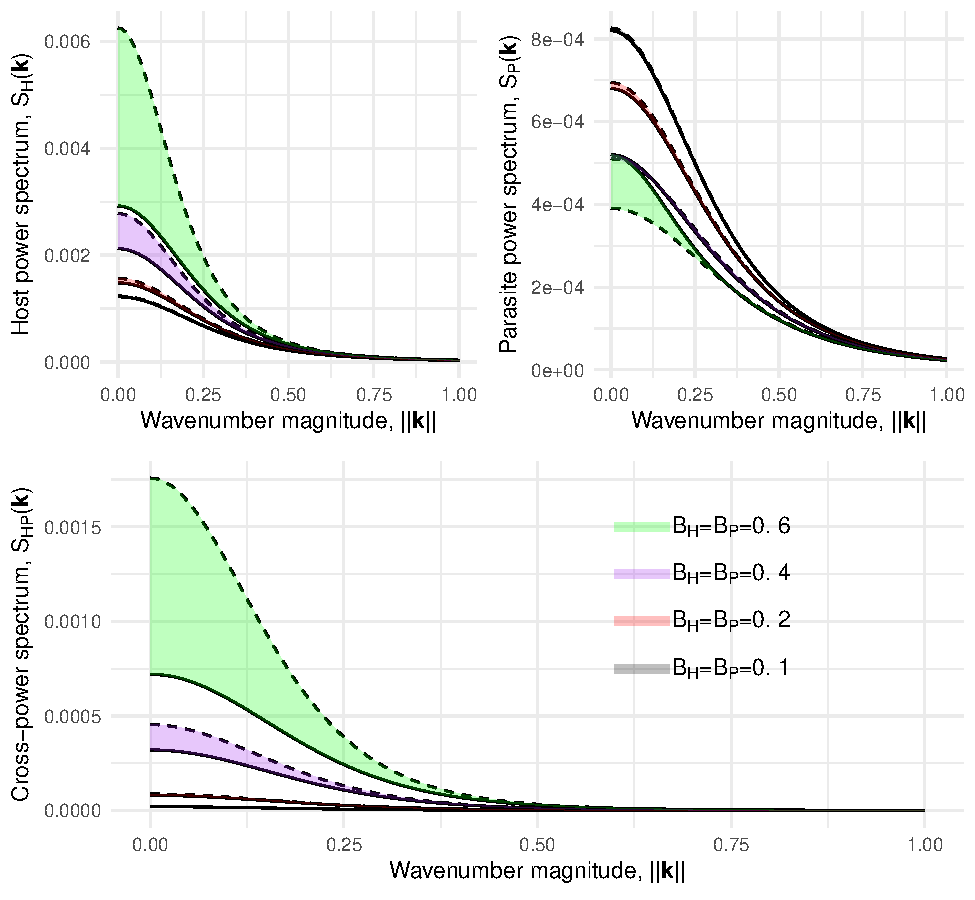
\includegraphics{Spatial-Scales-of-Local-Adaptation-in-Host-Parasite-Coevolution_files/figure-latex/unnamed-chunk-1-1.pdf}
\caption{Comparisons of approximated power spectra (dashed lines) to
exact power spectra (solid lines) for four different strengths of biotic
(coevolutionary) selection \(B=0.1,0.2,0.4,0.6\). For simplicity, biotic
selection on host and parasite are set equal (\(B_H=B_P=B\)). Background
parameters are set to \(A_H=A_P=1\), \(G_H=G_P=10\),
\(\sigma_H=\sigma_P=10\) and \(N_H=N_P=100\). Our model only is defined
for \(B_H<A_H\). Hence, the behaviour of power spectra as \(B\)
increases reflects what happens when the host comes closer to being able
to overcome abiotic stabilizing selection and escape parasitism. In this
limit, we see that our approximations over estimate the magnitudes of
low frequency content in the host spatial covariance and host-parasite
cross-covariance. This implies that our approximations over estimate the
spatial scale of phenotypic covariance of the host and phenotypic
cross-covariance of the host and parasite when coevolution is strong. In
contrast, we see that our approximations under estimate the amount of
low frequency content in the spatial covariance of parasite traits. This
implies that our approximations under estimate the spatial scale of
phenotypic covariance of the parasite when coevolution is strong.
However, when coevolution is relatively weak, say one-tenth the strength
of abiotic selection, we see our approximation matches closely the exact
power spectra.}
\end{figure}

To simplify notation, we denote by \(\xi_S\) the characteristic scale of
spatial trait covariance within species \(S=H,P\) and by \(V_S\) the
marginal variance of the same species. The marginal variance \(V_S\) can
be thought of as a measure of uncertainty when observing local mean
traits. Setting

\[\xi_H=\frac{\sigma_H}{\sqrt{G_H(A_H-B_H)}}, \ \xi_P=\frac{\sigma_P}{\sqrt{G_P(A_P+B_P)}},\]

\[V_H=\frac{1}{N_H\sigma_H^2(A_H-B_H)}, \ V_P=\frac{1}{N_P\sigma_P^2(A_P+B_P)},\]

the approximated power spectra can be rewritten as

\[S_H(\pmb k)\approx \frac{V_H\xi_H^2}{(1+\frac{1}{2}\xi_H^2\|\pmb k\|^2)^2}, \ S_P(\pmb k)\approx \frac{V_P\xi_P^2}{(1+\frac{1}{2}\xi_P^2\|\pmb k\|^2)^2}\]

\[S_{HP}(\pmb k)\approx \frac{B_P}{A_P+B_P}\frac{1}{1+\frac{1}{2}\xi_P^2\|\pmb k\|^2}\frac{V_H\xi_H^2}{(1+\frac{1}{2}\xi_H^2\|\pmb k\|^2)^2}-\frac{B_H}{A_H-B_H}\frac{1}{1+\frac{1}{2}\xi_H^2\|\pmb k\|^2}\frac{V_P\xi_P^2}{(1+\frac{1}{2}\xi_P^2\|\pmb k\|^2)^2}.\]

The spatial covariance functions, equal to the inverse Fourier
transforms of the power spectra
\(S_H(\pmb k),S_P(\pmb k),S_{HP}(\pmb k)\), can then be approximated as

\[C_H(\pmb x)\approx V_H\sqrt2\frac{\|\pmb x\|}{\xi_H}K_1\left(\sqrt2\frac{\|\pmb x\|}{\xi_H}\right),\]

\[C_P(\pmb x)\approx V_P\sqrt2\frac{\|\pmb x\|}{\xi_P}K_1\left(\sqrt2\frac{\|\pmb x\|}{\xi_P}\right),\]

where \(K_\nu\) is a modified Bessel function of the second kind, order
\(\nu\). Conveniently, the approximated spatial covariance functions
take the form of Whittle-Matérn covariance functions, which are widely
applied in the fields of spatial statistics (refs) and machine learning
(ref). In general, the Whittle-Matérn covariance function takes the form

\[M_\nu(\pmb x|\xi,V)=V\frac{2^{1-\nu}}{\Gamma(\nu)}\left(\sqrt{2\nu}\frac{\|\pmb x\|}{\xi}\right)^\nu K_\nu\left(\sqrt{2\nu}\frac{\|\pmb x\|}{\xi}\right).\]

Hence, \(C_S(\pmb x)=M_1(\pmb x|\xi_S,V_S)\) for both \(S=H,P\). With
this notation, the interspecific spatial cross-covariance function can
be approximated by

\[C_{HP}(\pmb x)\approx \int_{\mathbb R^2}\frac{2B_P}{A_P+B_P}\frac{K_0(\|\pmb y\|/\xi_P)}{\xi_P^2}M_1(\pmb x-\pmb y|\xi_H,V_H)-\frac{2B_H}{A_H-B_H}\frac{K_0(\|\pmb y\|/\xi_H)}{\xi_H^2}M_1(\pmb x-\pmb y|\xi_P,V_P)d\pmb y.\]

\hypertarget{marginal-values-and-integrals-of-spatial-covariance-and-cross-covariance-functions}{%
\subsection{Marginal values and integrals of spatial covariance and
cross-covariance
functions}\label{marginal-values-and-integrals-of-spatial-covariance-and-cross-covariance-functions}}

Following results from section A, the marginal covariance of species
mean traits can be approximated via

\[C_{HP}(\pmb 0)=\frac{1}{2\pi}\int_{\mathbb R^2}S_{HP}(\pmb k)d\pmb k\]

\[\approx \frac{G_HG_P}{\sigma_H^2\sigma_P^2}\frac{\xi_H^2\xi_P^2}{(\xi_H^2-\xi_P^2)^2}\left[\frac{B_P}{N_H\sigma_H^2}\Big(\xi_H^4+\xi_H^2\xi_P^2(\ln\xi_P^2-\ln\xi_H^2-1)\Big)\right.\]

\[\left.-\frac{B_H}{N_P\sigma_P^2}\Big(\xi_P^4+\xi_H^2\xi_P^2(\ln\xi_H^2-\ln\xi_P^2-1)\Big)\right].\]

Similarly, the integral of \(C_{HP}(\pmb x)\) is approximated via

\[\int_{\mathbb R^2}C_{HP}(\pmb x)d\pmb x=2\pi S_{HP}(\pmb 0)\approx2\pi \left(\frac{B_P}{G_HN_H(A_H-B_H)^2(A_P+B_P)}-\frac{B_H}{G_PN_P(A_H-B_H)(A_P+B_P)^2}\right)\]

\[=2\pi\left(\frac{B_PV_H\xi_H^2}{A_P+B_P}-\frac{B_HV_H\xi_H^2}{A_H-B_H}\right).\]

However, the integral \(\int_{\mathbb R^2}C_{HP}(\pmb x)d\pmb x\) is
biased by larger distances. To see this we can change our integration to
polar coordinates to find
\(\int_{\mathbb R^2}C_{HP}(\pmb x)d\pmb x=2\pi\int_0^\infty C_{HP}(r)rdr\).
To remove this bias, we should like to calculate
\(\int_0^\infty C_{HP}(r)dr\). Switching this integral back to Cartesian
coordinates yields

\[\int_0^\infty C_{HP}(r)dr=\frac{1}{2\pi}\int_{\mathbb R^2}\frac{1}{\|\pmb x\|}C_{HP}(\pmb x)d\pmb x.\]

To evaluate \(\int_0^\infty C_{HP}(r)dr\), we can use the relationship

\[\int_{\mathbb R^2}\frac{1}{\|\pmb x\|}C_{HP}(\pmb x)d\pmb x=\mathcal F\left\{\frac{C_{HP}(\pmb x)}{\|\pmb x\|}\right\}_{\pmb k=\pmb 0},\]

where \(\mathcal F\) denotes Fourier transformation and the subscript
denotes evaluation at \(\pmb k=\pmb 0=(0,0)^\top\). Taking the Fourier
transform of \(C_{HP}(\pmb x)/\|\pmb x\|\), we find

\[\mathcal F\left\{\frac{C_{HP}(\pmb x)}{\|\pmb x\|}\right\}\approx\frac{B_P}{A_P+B_P}\frac{1}{1+\frac{1}{2}\xi_P^2\|\pmb k\|^2} \frac{V_H\xi_H/\sqrt2}{1+\frac{1}{2}\xi_H^2\|\pmb k\|^2}E\left(-\frac{1}{2}\xi_H^2\|\pmb k\|^2\right)\]

\[-\frac{B_H}{A_H-B_H}\frac{1}{1+\frac{1}{2}\xi_H^2\|\pmb k\|^2} \frac{V_P\xi_P/\sqrt2}{1+\frac{1}{2}\xi_P^2\|\pmb k\|^2}E\left(-\frac{1}{2}\xi_P^2\|\pmb k\|^2\right),\]

where \(E(\zeta)=\int_0^{\pi/2}\sqrt{1-\zeta\sin^2\theta}d\theta\) is an
elliptic integral. In particular, this provides

\[\mathcal F\left\{\frac{C_{HP}(\pmb x)}{\|\pmb x\|}\right\}_{\pmb k=\pmb 0}\approx\frac{\pi}{2}\left(\frac{B_P}{A_P+B_P}\frac{\xi_H}{\sqrt2}-\frac{B_H}{A_H-B_H}\frac{\xi_P}{\sqrt2}\right).\]

We therefore conclude

\[\int_0^\infty C_{HP}(r)dr\approx\frac{1}{4}\left(\frac{B_P}{A_P+B_P}\frac{\xi_H}{\sqrt2}-\frac{B_H}{A_H-B_H}\frac{\xi_P}{\sqrt2}\right).\]

\hypertarget{measures-of-local-adaptation}{%
\section{\texorpdfstring{Measures of local adaptation
\label{la-app}}{Measures of local adaptation }}\label{measures-of-local-adaptation}}

\begin{itemize}
\tightlist
\item
  use \(\mathcal L\) for measures in terms of mean fitness and \(\ell\)
  for measures in terms of log-mean fitness
\end{itemize}

Local adaptation is commonly measured as the difference in fitness for
individuals experiencing their local environment and fitness for
individuals experiencing foreign environments (Gandon \& Nuismer 2009,
Nuismer 2017, etc). In the case of coevolution, the environmental
variable is replaced by the trait value of the interacting partner
species.

yada yada yada, folks end up with something like
\(\mathcal L_P=\tilde\alpha-\tilde\alpha_0\). Using a slightly different
definition, parasite local adaptation simplifies to
\(\ell_P=\widetilde{\ln\alpha}-\widetilde{\ln\alpha}_0=B_PC_{HP}(0)\).

Here extend this notion of local adaptation to the case of populations
distributed continuously in space. In particular, we denote by
\(\Delta_H(\pmb y)\) the difference in expected population growth rates
of the host when confronted with parasites drawn from a spatial lag
\(\pmb y=(y_1,y_2)^\top\) away. That is,

\[\Delta_H(\pmb y)=\mathbb E[m_H(\bar z_H(\pmb x),\bar z_P(\pmb x))-m_H(\bar z_H(\pmb x),\bar z_P(\pmb x+\pmb y))].\]

We define \(\Delta_P(\pmb y)\) in a complementary manner for the
parasite species. Under our model of trait matching/mis-matching,
\(\Delta_H(\pmb y)\) simplifies to

\[\Delta_H(\pmb y)=\mathbb E\left[\frac{B_H}{2}\left(\bar z_H(\pmb x)-\bar z_P(\pmb x)\right)^2-\frac{B_H}{2}\left(\bar z_H(\pmb x)-\bar z_P(\pmb x+\pmb y)\right)^2\right]=-B_HC_{HP}(\pmb y).\]

Similarly, we obtain \(\Delta_P(\pmb y)=B_PC_{HP}(\pmb y)\) for the
parasite. To provide a global measure of local adaptation, one that
accounts for all spatial distances, we might think
\(\invbreve{\ell}_S=\int_{\mathbb R^2}\Delta_S(\pmb y)d\pmb y\) would
provide a reasonable definition. Using our results from section A, we
obtain

\[\invbreve{\ell}_H\approx B_H\left(\frac{B_H}{G_PN_P(A_H-B_H)(A_P+B_P)^2}-\frac{B_P}{G_HN_H(A_H-B_H)^2(A_P+B_P)}\right),\]

\[\invbreve{\ell}_P\approx B_P\left(\frac{B_P}{G_HN_H(A_H-B_H)^2(A_P+B_P)}-\frac{B_H}{G_PN_P(A_H-B_H)(A_P+B_P)^2}\right).\]

These measures of local adaptation depend on the effective densities
\(N_H,N_P\) which suggests they provide some indication for the role of
random genetic drift in determining global patterns of local adaptation.
However, they are not dependent on dispersal distances because of the
extra weight given to larger distances implicit in this definition (see
above). Hence, they provide no information on the role of gene-flow in
determining global patterns of local adaptation. To circumvent this
issue, we define another index
\(\tilde{\ell}_S=\int_0^\infty\tilde\Delta_S(r)dr\) where
\(\tilde\Delta_S(r)=\Delta_S(\pmb r)\) and
\(\pmb r=(r/\sqrt2,r/\sqrt2)\). Using our results from above, we find

\[\tilde{\ell}_H\approx\frac{B_H}{4}\left(\frac{B_H}{A_H-B_H}\frac{\xi_P}{\sqrt2}-\frac{B_P}{A_P+B_P}\frac{\xi_H}{\sqrt2}\right),\]

\[\tilde{\ell}_P\approx\frac{B_P}{4}\left(\frac{B_P}{A_P+B_P}\frac{\xi_H}{\sqrt2}-\frac{B_H}{A_H-B_H}\frac{\xi_P}{\sqrt2}\right).\]

Since \(\xi_S\propto\sigma_S\) for \(S=H,P\) we see that this
alternative global index of local adaptation captures the role of
gene-flow. However, the absence effective densities in these expressions
suggests \(\tilde{\ell}_H,\tilde{\ell}_P\) do not capture the effects of
random genetic drift. Hence, the two sets of indices
\((\invbreve{\ell}_H,{\ell}_P)\) and \((\tilde{\ell}_H,\tilde{\ell}_P)\)
capture complementary aspects of global patterns of local adaptation in
coevolving hosts and parasites.

In particular, they both measure adaptation of a host (resp parasite)
when confronted with a randomly sampled parasite (resp host) drawn from
a randomly chosen location. However, the spatial sampling scheme differs
between the two. While \(\invbreve{\ell}\) samples space uniformly in
two-dimensions, \(\tilde{\ell}\) samples space uniformly along a
transect. Hence, while \(\invbreve{\ell}\) captures orientation, it is
sensitive to spatial dimension. In contrast, \(\tilde{\ell}\) focuses on
the effect of distance and we therefore focus on results for
\(\tilde{\ell}\) in the main text.

curious: does \(\invbreve{\ell}\) match the conditions for winner/loser
in the case of stochastic evolution without a spatial component?

\hypertarget{modified-index-of-local-adaptation-accounting-for-limited-dispersal}{%
\subsection{Modified Index of Local Adaptation Accounting for Limited
Dispersal}\label{modified-index-of-local-adaptation-accounting-for-limited-dispersal}}

We denote by \(D(\pmb x)\) the probability density that two individuals
of opposing species were separated by \(\pmb x\) before dispersal given
that they end up at the same location after dispersal. We refer to
\(D(\pmb x)\) as the separation kernel. Since we assume dispersal for
each species is bivariate Gaussian with respective standard deviations
(in both coordinates) \(\sigma_H,\sigma_P\), \(D(\pmb x)\) will also be
bivariate Gaussian with standard deviation
\(\sqrt{\sigma_H^2+\sigma_P^2}\).

Whereas local adaptation is classically measured as the difference
between fitness ``at home'' versus fitness in a randomly selected
environment, the limited dispersal analog is fitness ``at home'' versus
fitness in a randomly selected environment weighted by the separation
kernel. In particular, for species \(S=H,P\),

\[\invbreve{\mathcal L}_S=\mathbb E[\bar w_S(\pmb x,\pmb x)]-\mathbb E\left[\int_{\mathbb R^2}\bar w_S(\pmb x,\pmb x+\pmb y)D(\pmb y)d\pmb y\right],\]

where \(\bar w_H(\pmb x,\pmb y)\) and \(\bar w_P(\pmb x,\pmb y)\) are
shorthand for \(\bar w_H(\bar z_H(\pmb x),\bar z_P(\pmb y)\) and
\(\bar w_P(\bar z_P(\pmb x),\bar z_H(\pmb y))\) respectively. Applying
the trait matching/mis-matching model of fitness, we obtain

\[\invbreve{\mathcal L}_H=\cdots\]

\[\invbreve{\mathcal L}_P=\cdots\]

For the sake of clarity, we focus on a closely related measure of local
adaptation that utilizes the local population growth rate \(\bar m_S\)
instead of the population mean fitness \(\bar w_S\) for species
\(S=H,P\). In particular, we define

\[\invbreve\ell_S=\mathbb E[\bar m_S(\pmb x,\pmb x)]-\mathbb E\left[\int_{\mathbb R^2}\bar m_S(\pmb x,\pmb x+\pmb y)D(\pmb y)d\pmb y\right],\]

where \(\bar m_H(\pmb x,\pmb y)\) and \(\bar m_P(\pmb x,\pmb y)\) are
shortand for \(\bar m_H(\bar z_H(\pmb x),\bar z_P(\pmb y)\) and
\(\bar m_P(\bar z_P(\pmb x),\bar z_H(\pmb y))\) respectively. Applying
the trait matching/mis-matching model of fitness along with our
assumption of spatially homogeneous abiotic stabilizing selection, we
obtain

\begin{multline}
  \mathbb E[\bar m_H(\pmb x,\pmb x)]=
  r_H-\frac{A_H}{2}[(\theta_H-\mu_H)^2+v_H+V_H]
  +\frac{B_H}{2}[(\mu_H-\mu_P)^2+v_H+v_P+V_H+V_P] \\
  -B_HC_{HP}(0),
\end{multline}

\begin{multline}
  \mathbb E\left[\int_{\mathbb R^2}\bar m_H(\pmb x,\pmb y)
  D(\pmb y)d\pmb y\right]= 
  r_H-\frac{A_H}{2}[(\theta_H-\mu_H)^2+v_H+V_H] \\
  +\frac{B_H}{2}[(\mu_H-\mu_P)^2+v_H+v_P+V_H+V_P]
  -B_H\int_{\mathbb R^2}C_{HP}(\pmb y)D(\pmb y)d\pmb y,
\end{multline}

\begin{multline}
  \mathbb E[\bar m_P(\pmb x,\pmb x)]=
  r_P-\frac{A_P}{2}[(\theta_P-\mu_P)^2+v_P+V_P]
  -\frac{B_P}{2}[(\mu_P-\mu_H)^2+v_P+v_H+V_P+V_H] \\
  +B_P C_{HP}(0),
\end{multline}

\begin{multline}
  \mathbb E\left[\int_{\mathbb R^2}\bar m_P(\pmb x,\pmb y)
  D(\pmb y)d\pmb y\right]= 
  r_P-\frac{A_P}{2}[(\theta_P-\mu_P)^2+v_P+V_P] \\
  -\frac{B_P}{2}[(\mu_P-\mu_H)^2+v_P+v_H+V_P+V_H]
  +B_P\int_{\mathbb R^2}C_{HP}(\pmb y)D(\pmb y)d\pmb y,
\end{multline}

Setting \(\bar C_{HP}\int_{\mathbb R^2}C_{HP}(\pmb y)D(\pmb y)d\pmb y\),
the expressions for local adaptation accounting for limited dispersal
simplify to

\[\invbreve{\ell}_H=B_H\left(\bar C_{HP}-C_{HP}(0)\right),\]

\[\invbreve{\ell}_P=B_P\left(C_{HP}(0)-\bar C_{HP}\right).\]

\hypertarget{scotts-measure-of-coevolutionary-advantage}{%
\subsection{Scott's measure of coevolutionary
advantage}\label{scotts-measure-of-coevolutionary-advantage}}

\[\mathcal a=\bar{\bar m}-\bar{\bar m}^0\]

where \(\bar{\bar m}^0\) is the spatial average of growth rate in the
absence of biotic selection. Setting \(\bar{\bar z}_S^0, V_S^0\) the
spatial mean and variance of local mean traits for species \(S\) and
\(C_{HP}^{S,0}\) the covariance of mean traits between species when
\(B_S=0\), our model assumptions then implies

\begin{multline}
  \mathcal a_P=B_P(C_{HP}-C_{HP}^{P,0})-\frac{B_P}{2}\big[(\bar{\bar z}_H-\bar{\bar z}_P)^2+V_H+V_P+v_H+v_P\big] \\
  -\frac{A_P}{2}\big[(\theta_P-\bar{\bar z}_P)^2-(\theta_P-\bar{\bar z}_P^0)^2+V_P-V_P^0\big],
\end{multline}

\begin{multline}
  \mathcal a_H=-B_P(C_{HP}-C_{HP}^{H,0})+\frac{B_H}{2}\big[(\bar{\bar z}_P-\bar{\bar z}_H)^2+V_H+V_P+v_H+v_P\big] \\
  -\frac{A_H}{2}\big[(\theta_H-\bar{\bar z}_H)^2-(\theta_H-\bar{\bar z}_H^0)^2+V_H-V_H^0\big].
\end{multline}

\begin{itemize}
\tightlist
\item
  NOTE: Scott defines this measure by comparing the coevolutionary
  scenario to the no biotic selection for both species scenario. In this
  case it seems possible that \(\mathcal a\) can be positive for both
  species, blurring the distinction of which species is ``winning'' the
  coevolutionary race. Alternatively, we can proceed as above and
  consider the case when just one or the other species incurs zero
  biotic selection.
\end{itemize}

\hypertarget{relation-to-results-derived-without-gene-flow}{%
\subsection{Relation to results derived without
gene-flow}\label{relation-to-results-derived-without-gene-flow}}

Expressions for the spatial means, variance and covariance of local mean
traits across a set of discrete populations without gene-flow between
them have been presented by Week \& Nuismer (2019). In the model of Week
\& Nuismer (2019) coevolution was driven by an offset-matching mechanism
to capture trait escalation. When a parameter of their model known as
the optimal offset is set to zero, the classical trait-matching model is
recovered. Here we show how the results of Week \& Nuismer (2019) on the
spatial moments of a discrete space model with zero optimal offset are
recovered as a special case of the SPDE model presented here in the
limit of zero gene-flow (that is, in the limit of
\(\sigma_H,\sigma_P\to0\)). In this limit our SPDE model becomes

\[\dot{\bar z}_H=G_HA_H(\theta_H-\bar z_H)-G_HB_H(\bar z_P-\bar z_H)+\sqrt\frac{G_H}{N_H}\dot W_H,\]

\[\dot{\bar z}_P=G_PA_P(\theta_P-\bar z_P)+G_PB_P(\bar z_H-\bar z_P)+\sqrt\frac{G_P}{N_P}\dot W_P.\]

Without the homogenizing action of diffusive movement, solutions to this
equation become more technically involved. In particular, we no longer
have a function-valued equilibrium solution
\((\bar z_H,\bar z_P)^\top\). Instead, we work a more general notion
called a measure-valued solution. Whereas the function-valued solution
takes points in \(\mathbb R^2\) and returns normally distributed random
variables, the measure-valued solution takes subsets of \(\mathbb R^2\)
and returns normally distributed random variables.

To provide intuition for the measure-valued solutions, let us first
consider the case where \(\sigma_H,\sigma_P>0\) so that the equilibrium
function-valued solution \((\bar z_H,\bar z_P)^\top\) does in fact
exist. Then for bounded regions \(U\) of \(\mathbb R^2\) we can define

\[\bar Z_H(U)=\frac{1}{|U|}\int_U\bar z_H(x)dx, \ \ \bar Z_P(U)=\frac{1}{|U|}\int_U\bar z_P(x)dx,\]

where \(|U|\) denotes the area of the region \(U\subset\mathbb R^2\). In
this way, both \(\bar Z_H\) and \(\bar Z_P\) are random measures on
subsets of \(\mathbb R^2\) and thus constitute an equilibrium
measure-valued solution of the SPDE model.

Although the function-valued solution \((\bar z_H,\bar z_P)^\top\) fails
to exist in the absence of gene-flow (\(\sigma_H,\sigma_P=0\)), a
measure-valued solution \((\bar Z_H,\bar Z_P)^\top\) does exist. In
fact, for each fixed \(U\subset\mathbb R^2\) such that \(|U|<\infty\),
\((\bar Z_H(U),\bar Z_P(U))^\top\) correspond to equilibrium solutions
of a bivariate Ornstein-Uhlenbeck process. Following results presented
in Vatiwutipong and Phewchean (2019), the distribution of
\((\bar Z_H(U),\bar Z_P(U))^\top\) is bivariate normal determined by the
mean vector \(\pmb\mu=(\mu_H,\mu_P)^\top\) with

\[\mu_H=\frac{(A_P+B_P)A_H\theta_H-B_HA_P\theta_P}{(A_P+B_P)A_H-B_HA_P},\]

\[\mu_P=\frac{(A_H-B_H)A_P\theta_P+B_PA_H\theta_H}{(A_H-B_H)A_P+B_PA_H},\]

and variance-covariance matrix
\(\pmb\Sigma=\left(\begin{smallmatrix}V_H & C_{HP} \\ C_{HP} & V_P\end{smallmatrix}\right)\)
with

\[V_H=\frac{\frac{1}{2N_H}-B_HC_{HP}}{A_H-B_H}, \ \ V_P=\frac{\frac{1}{2N_P}+B_PC_{HP}}{A_P+B_P}\]

\[C_{HP}=\frac{B_P(A_P+B_P)G_PN_P-B_H(A_H-B_H)G_HN_H}{2(A_HA_P+A_HB_P-A_PB_H)((A_H-B_H)G_H+(A_P+B_P)G_P)N_HN_P}.\]

This results correspond to the results found by Week \& Nuismer (2019)
when the optimal offset is set to zero. Hence, the statistical model of
Week \& Nuismer (2019) can be interpreted as a special case of the
continuous space model presented here in the limit of zero gene-flow.
Assuming weak coevolution so that \(B_H^2,B_P^2,B_HB_P\approx0\), we
recover the marginal variances of mean trait values found using the SPDE
with gene-flow. However, applying the same approximation to the
covariance \(C_{HP}\) does not return the marginal covariance found
using the SPDE model with gene-flow. Hence, the presence of gene-flow
and limited dispersal fundamentally alters patterns of spatial trait
covariance between coevolving species.

\hypertarget{the-individual-based-model}{%
\section{\texorpdfstring{The individual-based model
\label{ibs-app}}{The individual-based model }}\label{the-individual-based-model}}

\newpage

\hypertarget{references}{%
\section*{References}\label{references}}
\addcontentsline{toc}{section}{References}

\hypertarget{refs}{}
\begin{CSLReferences}{1}{0}
\leavevmode\hypertarget{ref-Julia-2017}{}%
Bezanson, Jeff, Alan Edelman, Stefan Karpinski, and Viral B Shah. 2017.
{``Julia: A Fresh Approach to Numerical Computing.''} \emph{SIAM
{R}eview} 59 (1): 65--98. \url{https://doi.org/10.1137/141000671}.

\leavevmode\hypertarget{ref-Bjrnstad2001}{}%
Bjørnstad, Ottar N., and Jordi Bascompte. 2001. {``Synchrony and
Second-Order Spatial Correlation in Host-Parasitoid Systems.''}
\emph{Journal of Animal Ecology} 70 (6): 924--33.
\url{https://doi.org/10.1046/j.0021-8790.2001.00560.x}.

\leavevmode\hypertarget{ref-Vatiwutipong2019}{}%
Vatiwutipong, P., and N. Phewchean. 2019. {``Alternative Way to Derive
the Distribution of the Multivariate Ornstein-Uhlenbeck Process.''}
\emph{Advances in Difference Equations} 2019 (1).
\url{https://doi.org/10.1186/s13662-019-2214-1}.

\end{CSLReferences}

\bibliographystyle{unsrt}
\bibliography{references.bib}


\end{document}
